              
                %%%%%%%%%%%%%%%%%%%%%%%%%%%%%%%%%%%%%%%%%%%%%%%%%%%%%%%%%%%%%%%%%%%%%%
% LaTeX Example: Project Report
%
% Source: http://www.howtotex.com
%
% Feel free to distribute this example, but please keep the referral
% to howtotex.com
% Date: March 2011 
% 
%%%%%%%%%%%%%%%%%%%%%%%%%%%%%%%%%%%%%%%%%%%%%%%%%%%%%%%%%%%%%%%%%%%%%%
% How to use writeLaTeX: 
%
% You edit the source code here on the left, and the preview on the
% right shows you the result within a few seconds.
%
% Bookmark this page and share the URL with your co-authors. They can
% edit at the same time!
%
% You can upload figures, bibliographies, custom classes and
% styles using the files menu.
%
% If you're new to LaTeX, the wikibook is a great place to start:
% http://en.wikibooks.org/wiki/LaTeX
%
%%%%%%%%%%%%%%%%%%%%%%%%%%%%%%%%%%%%%%%%%%%%%%%%%%%%%%%%%%%%%%%%%%%%%%
% Edit the title below to update the display in My Documents
%\title{Project Report}
%
%%% Preamble
\documentclass[paper=letter, fontsize=11pt]{scrartcl}
\usepackage{url}
\usepackage{color}
\usepackage{fourier}
\usepackage{listings}
\usepackage[T1]{fontenc}
\usepackage[spanish]{babel}
\selectlanguage{spanish}
\usepackage{hyperref}
\usepackage[pdftex]{graphicx}
\usepackage[margin=2.5cm]{geometry}
\usepackage{amsmath,amsfonts,amsthm} % Math packages
                                       % English language/hyphenation
\usepackage[protrusion=true,expansion=true]{microtype}  

%%% Maketitle metadata
\newcommand{\horrule}[1]{\rule{\linewidth}{#1}}     % Horizontal rule

\title{
        %\vspace{-1in}  
        \usefont{OT1}{bch}{b}{n}
        \normalfont \normalsize \textsc{Universidad de los Andes, Departamento de F\'isica \\
        F\'isica at\'omica} \\ [25pt]
        \horrule{0.5pt} \\[0.4cm]
        \huge \'Atomo de hidr\'ogeno \\
        \horrule{2pt} \\[0.5cm]
}
\author{
        \normalfont                                 \normalsize
        Juan Barbosa, 201325901\\[-3pt]      \normalsize
        Marzo 07, 2017
}
\date{}

\lstset{keywordstyle=\color{blue}, basicstyle=\scriptsize, frame=single, language=Python}

%%% Begin document
\begin{document}
\maketitle

\[
\boxed{-\dfrac{\hbar^2}{2m}\nabla^2\Psi(x) + V(x)\Psi(x) = E\Psi(x)}
\]

Para el \'atomo de hidr\'ogeno la ecuaci\'on anterior se escribe usando coordenedas esf\'ericas, cuyo potencial depende de la parte radial:
\begin{equation}
	V(r) = \dfrac{ze^2}{4\pi\epsilon_0r}
\end{equation}

Usando separaci\'on de variable $\Psi(r, \theta, \phi) = R(r)\Theta(\theta)\Phi(\phi)$, la ecuaci\'on diferencial para $R$ se escribe:
\begin{equation}
	\dfrac{d^2R}{dr^2} + \dfrac{2}{r}\dfrac{dR}{dr} + \dfrac{2\mu}{\hbar^2}\left(E - \dfrac{ze^2}{4\pi\epsilon_0r}\right)R - \dfrac{l(l+1)}{r^2}R = 0
	\qquad \text{donde} \qquad l\in\mathbb{Z}	
\end{equation}

Haciendo un cambio de variable $r=\dfrac{a_0}{z}u$ se puede reescribir la ecuaci\'on anterior como:
\begin{equation}
	\dfrac{d^2R}{du^2}\left(\dfrac{z}{a_0}\right)^2 + \dfrac{2}{u}\dfrac{dR}{du}\left(\dfrac{z}{a_0}\right)^2+\dfrac{2\mu}{\hbar^2}\left(E - \dfrac{ze^2}{4\pi\epsilon_0u}\dfrac{z}{a_0}\right)R - \dfrac{l(l+1)}{u^2}R\left(\dfrac{z}{a_0}\right)^2 = 0
\end{equation}

Usando como factor com\'un $z^2/a_0^2$:
\begin{equation}
	\dfrac{d^2R}{du^2} + \dfrac{2}{u}\dfrac{dR}{du} + \dfrac{2\mu a_0^2}{\hbar^2z^2}\left(E - \dfrac{z^2e^2}{4\pi\epsilon_0ua_0}\right)R - \dfrac{l(l+1)}{u^2}R = 0
\end{equation}

Asumiendo $2\mu a_0^2/(\hbar^2z^2) = 1/E_0$
\begin{equation}
	\dfrac{d^2R}{du^2} + \dfrac{2}{u}\dfrac{dR}{du} + \left(\dfrac{E}{E_0} - \dfrac{z^2e^2}{4\pi\epsilon_0ua_0E_0}\right)R - \dfrac{l(l+1)}{u^2}R = \dfrac{d^2R}{du^2} + \dfrac{2}{u}\dfrac{dR}{du} + \left(\epsilon - \dfrac{2}{u}\right)R - \dfrac{l(l+1)}{u^2}R = 0
\end{equation}
\begin{equation}
	\dfrac{d^2R}{du^2} + \dfrac{2}{u}\dfrac{dR}{du} + \left(\epsilon - \dfrac{2}{u} - \dfrac{l(l+1)}{u^2}\right)R = 0
\end{equation}

Usando el m\'etodo de Euler para resolver num\'ericamente se obtiene:
\begin{equation}
	\begin{matrix}
	\dot{R}_n = \dot{R}_{n-1} + \ddot{R}_{n-1}\Delta u \qquad \text{donde} \qquad \ddot{R}_{n-1} = -\dfrac{2}{u}\dot{R}_{n-1} - \left(\epsilon - \dfrac{2}{u} - \dfrac{l(l+1)}{u^2}\right)R_{n-1} \\
	R_n = R_{n-1} + \dot{R}_n\Delta u
	\end{matrix}
\end{equation}

El sistema de ecuaciones diferenciales es resuelto con $N = 1000$ puntos, $dx = 0.1$, para $l = 0, 1, 2, 3$. Para $l = 0$ se usa como condiciones iniciales $R'(0) = -1$ y $R(0) = 1$, para todas las demas se usa $R'(0) = 1$ y $R(0) = 0$. El algoritmo funciona de forma analoga a el m\'etodo de bisecci\'on para encontrar ra\'ices.

\lstinputlisting{finder.py}
\newpage
\begin{figure}[ht]
	\centering
	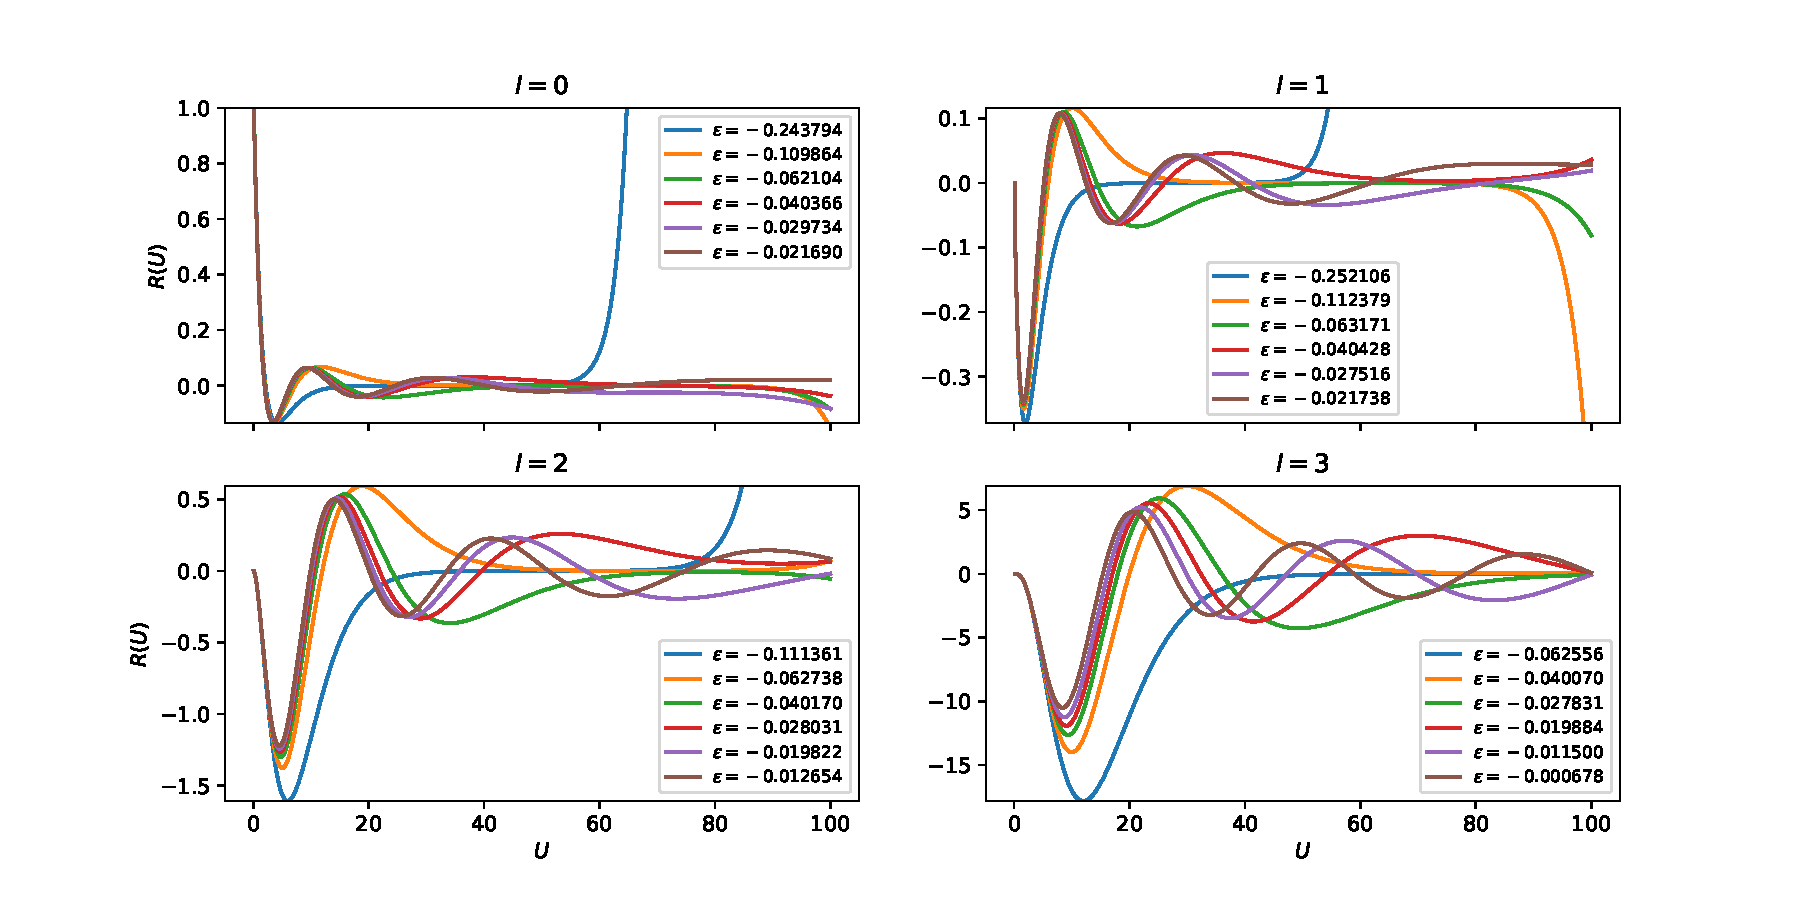
\includegraphics[width=\linewidth]{R.pdf}
	\caption{Primeros 6 valores de energ\'ia para $l = 0, 1, 2, 3$.}
	\label{fig:functions}
\end{figure}

\begin{table}[h]
	\centering
	\caption{Energ\'ias obtenidas para los distintos valores de $l$ ordenadas en niveles $n$, el valor te\'orico esperado corresponde con $\epsilon_T$.}
	\begin{tabular}{cccccc}
		\hline
		$n$ & $\epsilon_T$ & $\epsilon_{l=0}$ & $\epsilon_{l=1}$ & $\epsilon_{l=2}$ & $\epsilon_{l=3}$ \\
		\hline
		2 & -0.250000 & -0.243793716 & -0.252106231851 &  &  \\
		3 & -0.111111 & -0.109863584471 & -0.112379400942 & -0.111360953653 &  \\
		4 & -0.062500 & -0.0621041237279 & -0.0631713802996 & -0.0627381968616 & -0.0625562074569 \\
		5 & -0.040000 & -0.0403662521966 & -0.0404282449355 & -0.0401698413622 & -0.0400696123192 \\
		6 & -0.027778 & -0.0297344023873 & -0.0275164742092 & -0.028031058596 & -0.0278314836864 \\
		7 & -0.020408 & -0.0216904640572 & -0.0217380146253 & -0.0198219628643 & -0.0198838400997 \\
		8 & -0.015625 &  &  & -0.0126540207376 & -0.0115004356954 \\
		9 & -0.012346 &  &  &  & -0.000678129139279 \\
		\hline
	\end{tabular}
	\label{tb: table}
\end{table}

En la \autoref{fig:functions} se muestra las funciones $R$ para las cuales se considera convergencia existe un cambio en el signo de la pendiente entre ellas y un $d\epsilon$. Las funciones son simuladas de $u=0$ hasta $u=100$. En el \autoref{tb: table} se muestran los primeros seis valores de energ\'ia obtenidos para distintos valores de $l$. Se observa que los valores de $l$ son estrictamente menores a $n$. Adicionalmente se obtiene aproximadamente la misma energ\'ia para un mismo $n$ y distinto $l$.

En la \autoref{fig:prop} se muestran las funciones de probabilidad para las distintas funciones $R_{l,n}(u)$. La probabilidad se encuentra normalizada, esto es que:
\begin{equation}
	P = \dfrac{P}{\int Pdu}
\end{equation}
En ellas se observa que la probabilidad de encontrar el electr\'on a distancias grandes aumenta con la energ\'ia del mismo. Tambi\'en se puede ver que el m\'aximo existe para el valor m\'inimo de $n$ que puede soportar $l$, es decir $n = l-1$.

\begin{figure}[!ht]
	\centering
	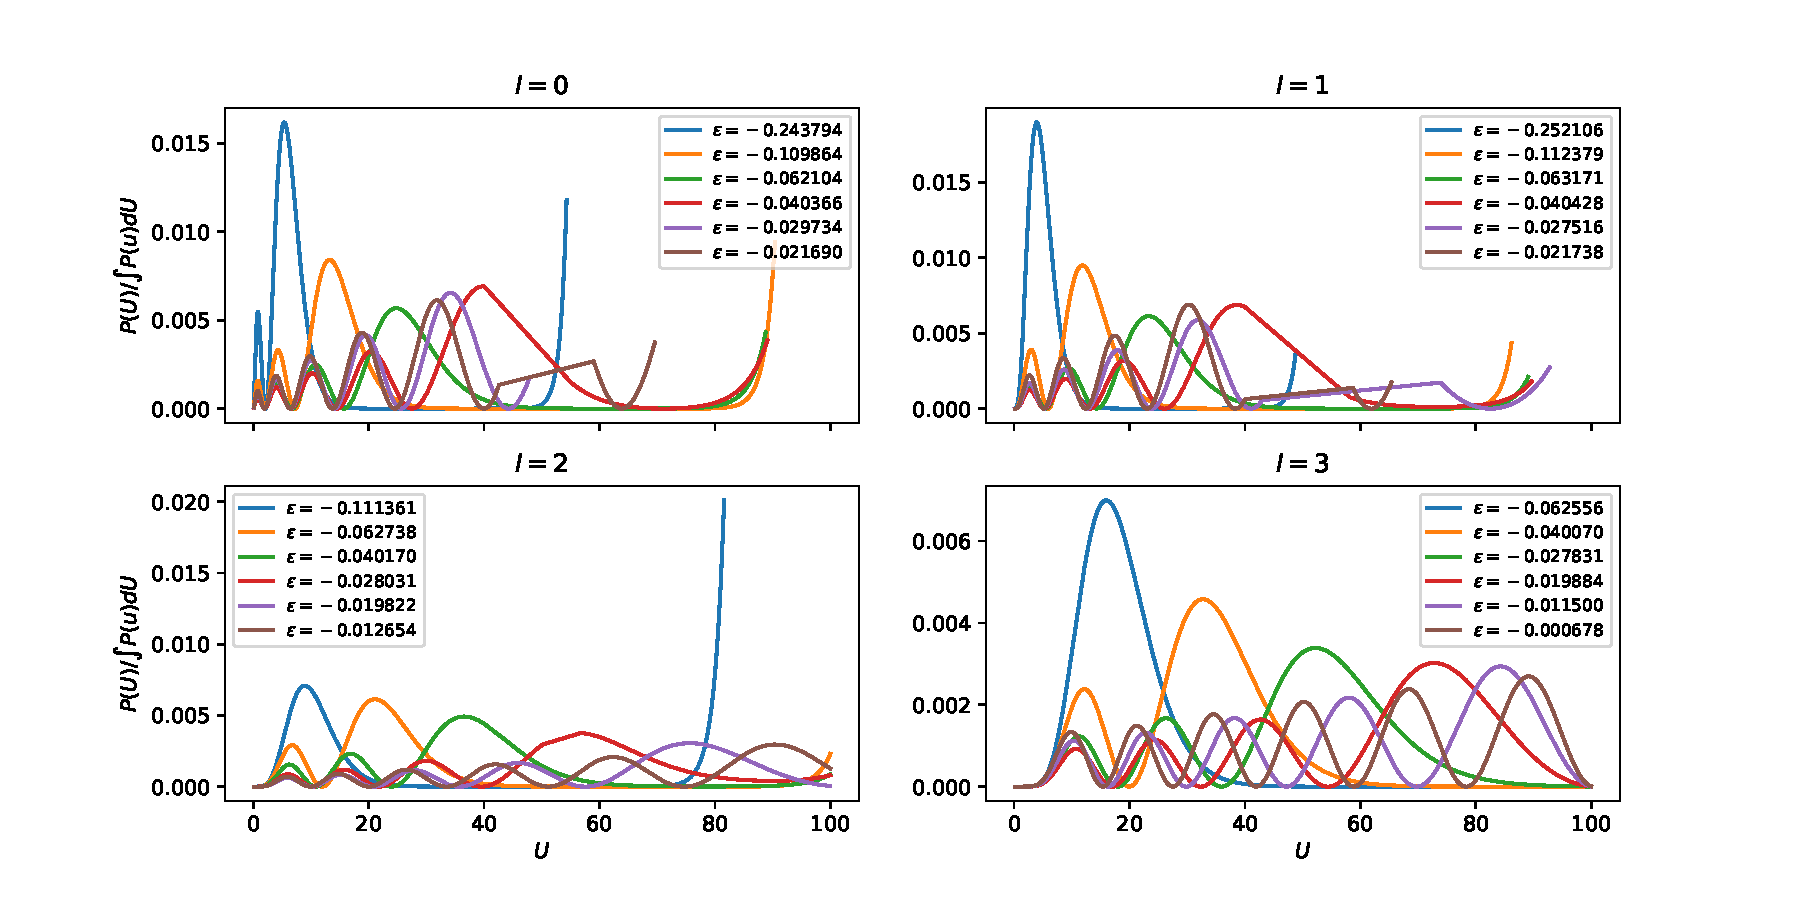
\includegraphics[width=\linewidth]{P.pdf}
	\caption{Funci\'on normalizada de probabilidad. Para distintos valores de $\epsilon$ y $l$.}
	\label{fig:prop}
\end{figure}
\end{document}
              